% <<<<<< Rapport projet de troisième année >>>>>>

\documentclass[a4paper,12pt,titlepage]{report}
\usepackage[utf8]{inputenc}
\usepackage[T1]{fontenc}
\usepackage{lmodern}
\usepackage[a4paper]{geometry}
\usepackage[french]{babel}
\usepackage{amsmath}
\usepackage{amssymb}
\usepackage{mathrsfs}

\usepackage{graphicx}
\usepackage{appendix}
\usepackage{hyperref}
\usepackage{subcaption}
\usepackage{setspace}
\usepackage[intoc]{nomencl}
%\usepackage{algorithm}
%\usepackage{listing}
\usepackage{verbatim}

\begin{document}


%==================================== Page de Garde ==============================
\begin{titlepage}
 
	\begin{center}
	\begin{figure}[!h]
	\centering	
		\begin{subfigure}[b]{0.3\textwidth}
		
\includegraphics[height = 2cm, keepaspectratio]{graphes/mines_nancy.png}
		\end{subfigure}
		\begin{subfigure}[b]{0.3\textwidth}
		
\includegraphics[height = 2cm, keepaspectratio]{graphes/elie_cartan.png}
		\end{subfigure}
		\begin{subfigure}[b]{0.3\textwidth}
		
\includegraphics[height = 2cm, keepaspectratio]{graphes/univ_lorraine.png}
	\end{subfigure}
	\end{figure}
 
	\textsc{École nationale supérieure des Mines de Nancy}\\[2cm]
	\textsc{Rapport de projet 3A}\\[1cm]
	\textsc{Pierre Gauthier}\\[1cm]
 
	\begin{doublespace}
		{ \huge \bfseries{Algorithme d'apprentissage en chimie quantique et application au screening (sélection) de cellules photovoltaïques}}\\[2cm]
	\end{doublespace}
	\textmd{Laboratoire : Institut Élie Cartan}\\[1cm]
	\textmd{Tuteurs : Dario Rocca et Marianne Clausel}
	% Bottom of the page
	\vfill
	{\textit{{\large 21 Novembre 2018}}}
 
	\end{center}
\end{titlepage}

%================= Table des matières ===============================
\tableofcontents

\newpage



%======================== Introduction ==============================
\textbf{\Huge Introduction:} \\
\newline

Ce projet est conduit dans un cadre pédagogique en tant que projet de troisième année à l'Ecole des Mines de Nancy. Il suit la publication scientifique de Mathias Rupp "Machine Learning for Quantum Mechanics in a Nutshell". Dans cette publication Mathias Rupp propose d'allier la mécanique quantique aux méthodes de machines learning pour faire de la prédiction à partir de données et ainsi dépasser les problèmes en terme de puissance de calcul du problème à N-corps. Il vise ainsi à prédire l'énergie d'atomisation de molécules à partir d'un set de données d'entrainement, en utilisant des méthode de  linéaire, notamment la régression à vecteur supports (SVM). 
Le premier objectif du projet est de reproduire les résultats de cette études, et d'explorer des variations dans les paramètres sur l'erreur finale de prédiction. Nous pourrons également dépasser le travail réaliser dans l'étude en travaillant sur des données avec de nouveaux descripteurs qui prennent en compte les propriétés des groupes chimiques des molécules.\\
Nous allons dans une première partie présenterer les méthodes à vecteur support avec l'astuce des noyaux.

%%%%%%%%%%%%%%%%%%%%%%%% Chapitre 1 %%%%%%%%%%%%%%%%%%%%%%%%%%%
\chapter{Théorie}
\label{C1}
%%%%%%%%%%%%%%%%%%%%%%%%% sectioon 1 %%%%%%%%%%%%%%%%%%%%%%%%%%%%%%
\section{Support Vector Machines methods (SVM}
Le probléme SVM vise à séparer les données $(x_{i},\ y_{i})_{1 \leqslant i \leqslant N},\ x_{i} \in \mathbb{R}, \ y_{i} \in \{-1,\ 1\}$ en deux classes $+1$ et $-1$ à l'aide de la fonction $f(x) = w \cdot x + b \ (b \in \mathbb{R},\ w \in  \mathbb{R}^{d})$ telle que $f(x) > 0 \Rightarrow x \in C_{+1}$, et $f(x) < 0 \Rightarrow x \in C_{-1}$

\begin{figure}[!h]
	\begin{center}
	\centering	
	%\begin{subfigure}[b]{0.3\textwidth}
		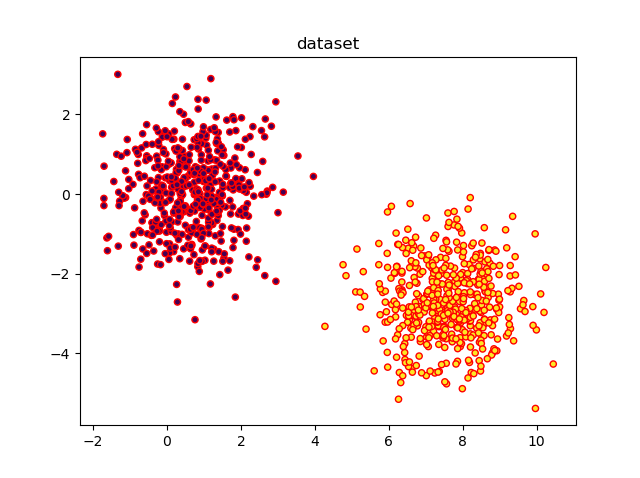
\includegraphics[height = 5cm, keepaspectratio]{graphes/SVM_donnee.png}
		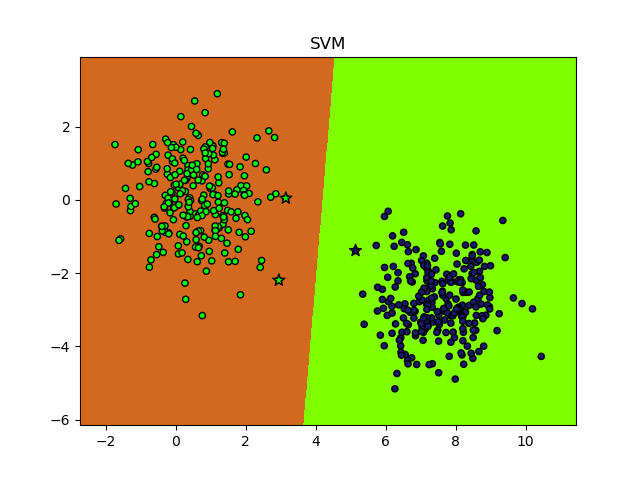
\includegraphics[height = 5cm, keepaspectratio]{graphes/SVM_separee.png}
		\caption{sparation de données générées make$\_$blobs du package dataset et séparation de l'espace en deux classe par la méthode des vecteurs support à l'aide de la fonction SVC du package sklearn. Les étoiles sont les vecteurs supports.}
			%\end{subfigure}
	\end{center}
\end{figure}
Nous voulons trouver l'hyperplan qui sépare le mieux nos données parmi tous ceux compatibles.

Pour juger la qualité d’un hyperplan en tant que séparateur on utilise la distance entre les exemples d’apprentissage et ce séparateur. Plus précisément, la « marge » d’un problème d’apprentissage est définie comme la distance entre le plus proche exemple d’apprentissage et l’hyperplan de séparation. \\
Pour un hyperplan $H$, On a :
\[
\text{Marge}(H) = \text{min}_{x_{i}}\ d(x_i,\ H)
\]
\begin{figure}[!h]
	\begin{center}
	\centering	
	%\begin{subfigure}[b]{0.3\textwidth}
		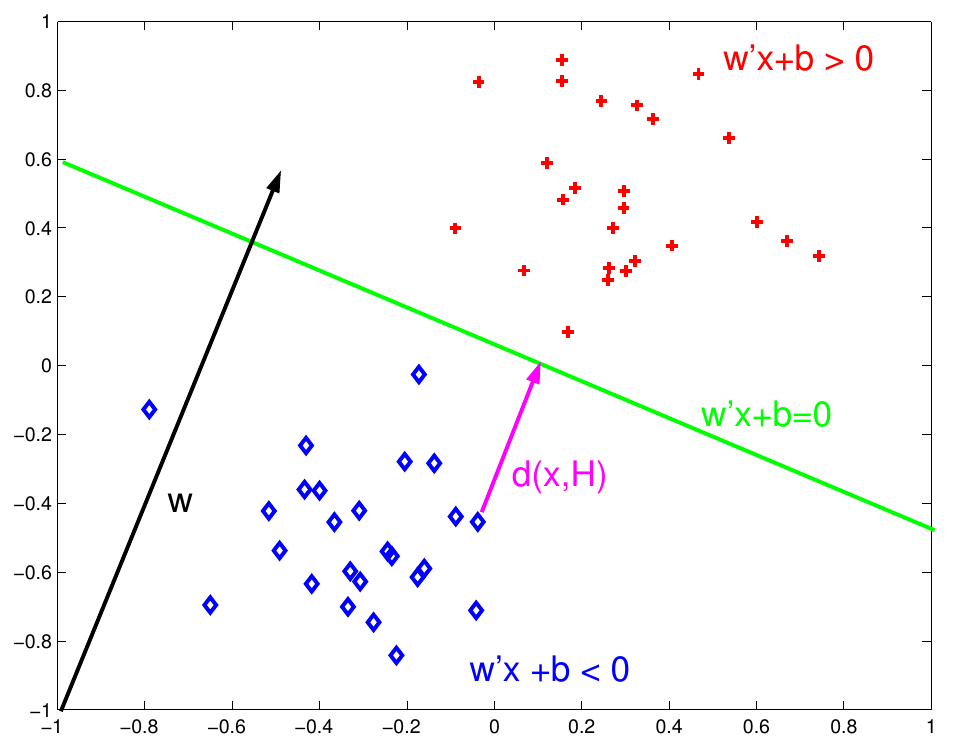
\includegraphics[height =6cm, keepaspectratio]{graphes/svm05.png}
		\caption{Le séparateur idéal correspond intuitivement à l’hyperplan qui passe « au milieu » entre les données sans préférence pour une classe ou une autre. C’est le séparateur de marge maximale.[Cours Cnam RCP209]}
			%\end{subfigure}
	\end{center}

Sous l'hypothèse qu'il exixte un hyperplan qui sépare nos données, trouver l'hyperplan qui maximise la marge revient à résoudre le problème suivant:
\[
	\left\{
	\begin{array}{ccc}		
	\begin{aligned}
		&\text{arg}\ \text{min}_{w,b}\ \frac{1}{2}||w||^{2} \\
		&\forall \ 1 \leqslant i \leqslant N,\ y_i (w \cdot x_i + b)\geqslant 1
	\end{aligned}
\end{array}
	\right.
% − \sum{ \lambda_{i} (y_{i} (w \cdot x_i + b)−1)}
\]

On utilise le lagrangien des conditions de Karush, Kuhn et Tucker, qui s'exprime sous la forme suivante :
\[
L(w,b,\lambda_{i}) = \frac{1}{2}||w||^{2} - \sum{\lambda_{i}( y_i (w \cdot x_i + b)-1)}
\]

On recherche donc le $\lambda$ qui maximise
\[
\text{max}\ L(\lambda) = \sum_{i}{\lambda_{i}} - \frac{1}{2} \sum_{i}{\sum_{j}{\lambda_{i} \lambda_{j} y_i y_j x_i \cdot x_j}} 
\]
\[
\text{sous contraintes}\ \lambda_i \geqslant 0 \  \text{et} \sum_{i}\lambda_i y_i = 0 
\]
\end{figure}

On utilise alors l'astuce du noyaux qui consiste à remplacer le produit scalaire $x \cdot y$
par un noyaux reproduisant $K(x,y) = \phi(x) \cdot \phi(y)$, $K :\xi \time \xi \rightarrow \mathbb{R}$, $\phi :\xi \rightarrow \mathbb{R}$  . Le théorème de Mercer assure l'existence d'une telle décomposition du noyaux $K$

\begin{figure}[!h]
	%\begin{center}
		
	%\begin{subfigure}[b]{0.3\textwidth}
		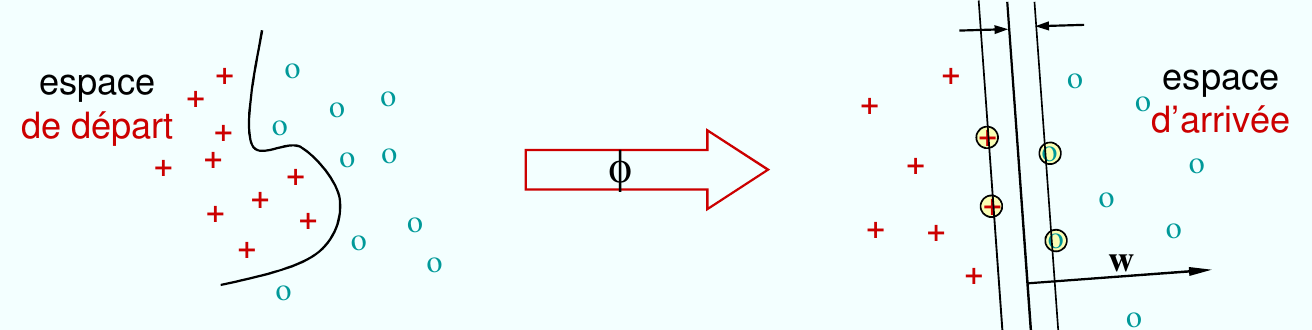
\includegraphics[height = 4cm, keepaspectratio]{graphes/mnoyaux05.png}
		\caption{Astuce à noyaux : projeter les données dans un espace de dimension beaucoup plus grande, où elles deviennent séparables linéairement.[Cours Cnam RCP209]}
			%\end{subfigure}
	%\end{center}
\end{figure}

L'estimateur devient ainsi en effectuant le produit scalaire sur les données $(x_{i})_{1 \leqslant i \leqslant N}$:
\[
f(\overset{\sim}{x}) = \sum_{i = 1}^{n}{\alpha_i \text{k}(x_i , \overset{\sim}{x})}
\]


%%%%%%%%%%%%%%%%%%% section 2 %%%%%%%%%%%%%%%%%%%%%%%%%%%%%%%%%%%%%%%%%%
\section{Ridge Regression}
%%%%%%%%%%%%%%%%%%%%%%%%%%%%%%%%%%%%%%%%%%%%%%%%%%%%%%%%%%%%%%%%%%%%%$

Le problème linéaire classique $Y = \sum{w_i \cdot x_i}$ est optimisé par minimisation de l'erreur :
\[
\underset{W \in \mathbb{R}^{n}}{\text{arg min}}\sum{(f(x_i) - y_i)^{2}}
\]
La regression ridge consiste à ajouter un poid à cette erreur avec un paramètre $\lambda\geqslant 0 $ :
\[
\underset{W \in \mathbb{R}^{n}}{\text{arg min}}\sum{(f(x_i) - y_i)^{2}} +  \lambda \sum{w_{i}^{2}}
\]
En reprenant l'astuce du noyaux précedente ce problème de minimisation peut se réécrire :
\[
	\underset{\alpha \in \mathbb{R}^{n}}{\text{arg min}}<K \alpha - y , K 	\alpha -y > + \lambda \alpha^{T} K \alpha 
\]
\[
	\text{où } K \in \mathbb{R}^{n \times n} \text{ est la matrice des 			noyaux} \quad K_{i,j} = \text{k}(x_i, x_j)
\]
ce qui revient en prenant le gradient à :
\[
\alpha	=(K + \lambda I)^{-1}y 
\]
\[
\text{avec $I$ la matrice identité}
\]

%%%%%%%%%%%%%%%%%%%%% chapitr 2 %%%%%%%%%%%%%%%%%%%%%%%%%%%%%%%%%%%%%%
\chapter{Experimentations}


%%%%%%%%%%%%%%%%%%%%%%%%%% SECTION 1 %%%%%%%%%%%%%%%%%%%%%%%
\section{Base d'entrainement du modèle}

Nos données sont initialement contenues dans un fichier .xyz.
Chaque élément du fichier est un tableau avec en première ligne le nombre d'atome de la molécule, en deuxième ligne l'énergie d'atomisation et le numéro de la molécule dans le fichier, et pour chaque ligne ensuite correspondantes à chaque atomes les coordonnées cartésienne de l'atome.\\
\\
\begin{tabular}{ l c c c }
   Nombre d'atome &  & & \quad\\
   numéro de la molécule &\quad énergie d'atomisation &\quad &\\
   atome 1 & x(1) & y(1) & \quad z(1) \\
   atome 2 & x(2) & y(2) & \quad z(2) \\
   . & . & . & \quad . \\
   . & . & . & \quad . \\
   . & . & . & \quad . \\
   atome n & x(n) & y(n) &\quad  z(n) \\
 \end{tabular}
 \\
 \\
 \\
 Par exemple pour la première  molécule du fichier que l'on traite :
\begin{figure}[!h]
\begin{tabular}{ l c c c c c c}
   5 &  & & \quad\\
   0001 &\quad -417.031 & & & & & \\
   C & 1.04168000 & -0.05620000 & -0.07148000 & 1.04168200 & -0.05620000 & -0.07148100\\
   H  & 2.15109000 & -0.05620000 & -0.07150000 & 2.13089400 & -0.05620200 & -0.07149600\\
   H  & 0.67187000 & 0.17923000 & -1.09059000  &  0.67859800 &  0.17494100 & -1.07204400\\
   H & 0.67188000 & 0.70866000 & 0.64196000 & 0.67861300 &  0.69474600  & 0.62898000\\
   H & 0.67188000 & -1.05649000 & 0.23421000 & 0.67861400 & -1.03828500  &0.22864100\\
 \end{tabular}
 \caption{Premier élément du fichier .xyz correspondant à la première molécule. Le bloc de coordonnées à gauche correspond aux coordonnées du champ de force et le bloc de droite correspond aux coordonnées DFT.}
 \end{figure}
 
 \newpage
Nous allons ensuite mettre en forme ces données pour entrainer le modèle. On utilise ainsi les matrices de Coulomb pour représenter les molécules.
Les matrices de Coulomb sont représentés comme suit : 
\[
M_{ij} = 
	\left\{
	\begin{array}{ccc}		
	\begin{aligned}
		& 0.5 Z_{i}^{2.4} \quad &i=j\\
		& \frac{Z_i Z_j}{||R_i - R_j||_{2}} \quad &i\neq j
	\end{aligned}
\end{array}
	\right.
\]
avec $Z_i$ le numéro atomique correspondant et $R_i$ la position des atomes.\\
Cependant pour chaque molécules les coordonnées des atomes sont déterminé par rapport à un atome de référence ce qui fait que ces matrices ne sont pas insensible à l'inversion de ligne pour l'entrainement du modèle. Pour ce la après le calcul des matrices nous trions les ligne par norme descendante.\\
De plus les matrices de Coulomb étant symétrique nous ne pouvons garder que la partie inférieure de la matrice dans un vecteur colonne de taille égale au plus grand vecteur possible sur nos données.

%%%%%%%%%%%%%%%%%% section 2%%%%%%%%%%%%%%%%%%%%%%%%%%%%%
\section{entraînement du modèle}

Nous allons dans un premier temps travailler avec un noyaux gaussien définis par :
\[ 
	\text{k}(x,z) = \exp{- \frac{||x-z||_{2}^2}{2\sigma^2}} \, \quad \sigma \geqslant 0 
\]
\\
Nous avons donc trois paramètres dans notre modèle d'après le chapitre\ref{C1} à la page \pageref{C1}
\begin{enumerate}
    \item $\sigma$ du noyaux gaussien
    \item $\lambda$ de la ridge régression
\end{enumerate}

Le vecteur $\alpha$ dans l'estimateur  $f(\overset{\sim}{x}) = \sum_{i = 1}^{n}{\alpha_i \text{k}(x_i , \overset{\sim}{x})}$ est directement déterminé
par $\alpha	=(K + \lambda I)^{-1}y$

nous allons ainsi rechercher directement le meilleur couple $(\lambda, \sigma)$ sur un ensemble $\Omega$ en mimisant l'erreur en utilisant la cross-validation. 
\end{document}
